\chapter{Parte III - Estilo do INPE}
\label{cap:parteIII}

O INPE desenvolveu um estilo próprio para a publicação de teses, dissertações e relatórios. Este estilo está disponível para edição na linguagem de marcação \LaTeX{}, além dos editores WYSIWYG \textit{Microsoft Word} e \textit{LibreOffice}. Este capítulo trata da aplicação do estilo do INPE no ambiente da linguagem de marcação \LaTeX{}.

\section{Estilo do INPE para Dissertações e Teses}

O estilo do INPE compreende um conjunto de arquivos que contém instruções e imagens, que permitem que os documentos escritos dentro do seu escopo, sejam renderizados segundo as normas de publicação do SID do INPE. O estilo do INPE foi originalmente criado por Banon (XXXX), e tem sido mantido e atualizado desde 2002. A versão mais atualizada do estilo, que inclui o logo do governo atual, é a versão v1.28, publicada em 8 de Junho de 2014. Nesta seção, esta é versão considerada do estilo.

\subsection*{Obtendo o Estilo}
\label{sec:obter}

É possível obter uma cópia do estilo do INPE a partir de duas formas distintas. A primeira, é entrar no \textit{site} da biblioteca do INPE, a partir do endereço \url{http://www.inpe.br/biblioteca/}. Na página, no menu lateral, clique em ``Como Publicar?'' e depois em ``em \LaTeX{}'' (Figura \ref{fig:biblio_pub_latex}). Na página, no \textit{frame} da direita, uma página irá se abrir com as instruções ``Publicar usando estilo em \LaTeX{}''. A página contém instruções sobre todo o processo de publicação de documentos submetidos à revisão pelo SID. Para obter uma cópia \textit{offline} do pacote com o estilo do INPE em \LaTeX{}, clique no link \href{http://mtc-m16c.sid.inpe.br/archive.cgi/sid.inpe.br/iris@1905/2005/08.25.14.01}{``download do estilo baixando o arquivo archive.zip''} que está na ``OPÇÃO 3 (compilação no próprio computador)''. Na mesma página, há instruções sobre a instalação de um compilador \LaTeX{}, que também podem ser encontradas no Capítulo \ref{cap:parteI} deste documento.

\begin{figure}[H]
    \centering
    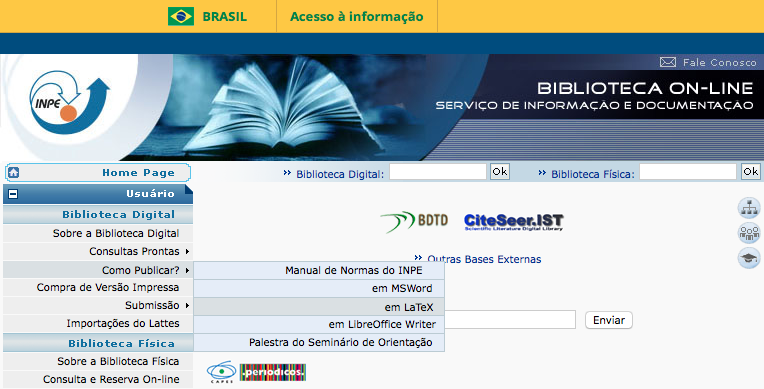
\includegraphics[scale=0.5]{./figs/biblio_pub_latex.png}
    \caption{Obtenção do estilo \LaTeX{} do INPE a partir do \textit{site} da Biblioteca do INPE.}
    \label{fig:biblio_pub_latex}
\end{figure}

Com o arquivo ``archive.zip'' no seu computador, descompacte-o em um local apropriado para poder ter acesso aos arquivos que compõem o estilo do INPE.

%\subsection{Conhecendo a estrutura e ambiente (arquivos que compõem o modelo, preenchimento de dados básicos, dicas práticas sobre o que se pode e o que não se pode fazer na hora de utilizar o modelo do INPE)}

\subsection{Estrutura e Organização}
\label{sec:estrut}

O estilo do INPE é fornecido pelo arquivo ``tdiinpevx-x.x.cls''. Dentro deste arquivo há uma série de instruções da linguagem \LaTeX{} que determinam o estilo das referências, dos capítulos, dos títulos, tabelas, imagens etc (Figura \ref{fig:estrut}).

\begin{figure}[H]
    \centering
    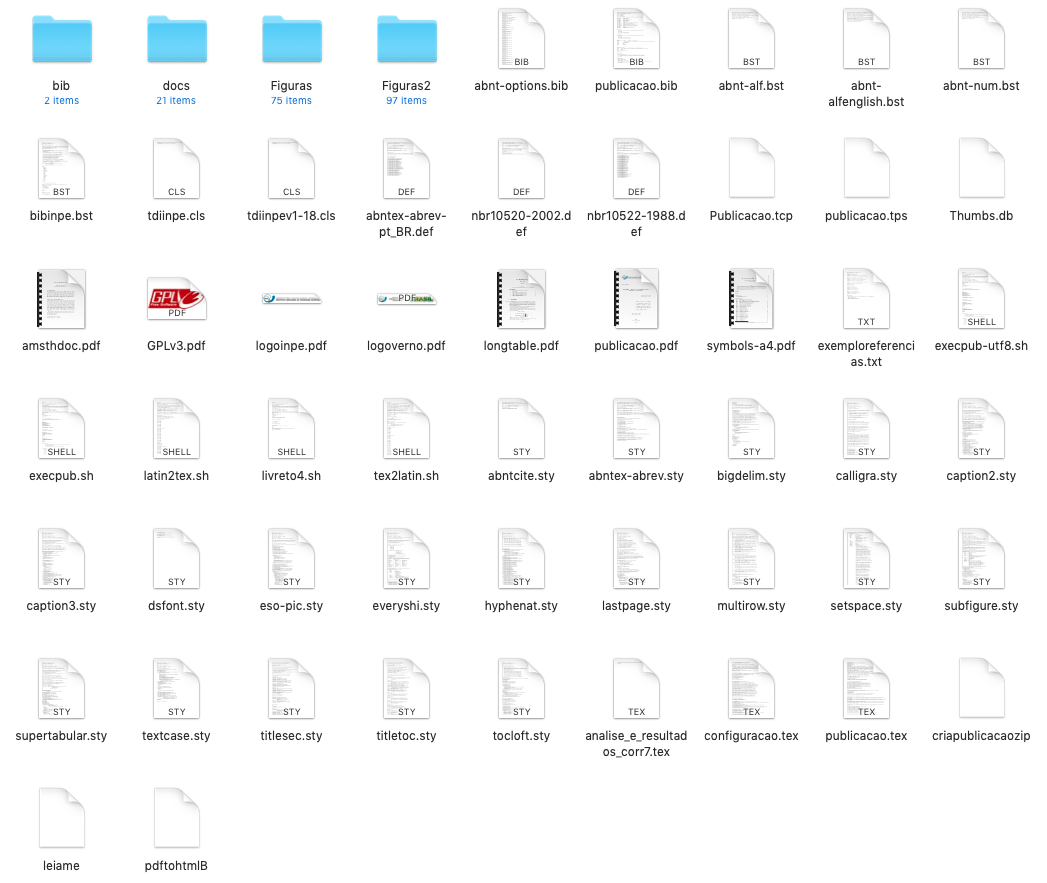
\includegraphics[scale=0.4]{./figs/estrutura_estilo_inpe.png}
    \caption{Estrutura e organização do estilo \LaTeX{} do INPE.}
    \label{fig:estrut}
\end{figure}

Na Figura \ref{fig:estrut}, os arquivos da estrutura do estilo do INPE estão misturado aos arquivos do documento em si. Outros arquivos são resultados do processo de compilação do documento principal.

\begin{multicols}{3}
    \textbf{Diretórios}
    \begin{itemize}
        \item bib/
        \item Figuras/
        \item Figuras2/
        \item docs/
    \end{itemize}
    \textbf{Arquivos do Estilo}
    \begin{itemize}
        \item leiame
        \item GPLv3.pdf
        \item abntex-abrev-pt\_BR.def
        \item caption3.sty
        \item hyphenat.sty
        \item multirow.sty
        \item CCBY.png
        \item abntex-abrev.sty
        \item configuracao.tex
        \item lastpage.sty
        \item nbr10520-2002.def
        \item textcase.sty
        \item CCBYNC.png
        \item amsthdoc.pdf
        \item nbr10522-1988.def
        \item setspace.sty
        \item titlesec.sty
        \item CCBYNCND.png
        \item subfigure.sty
        \item titletoc.sty
        \item CCBYNCSA.png
        \item abnt-alf.bst
        \item dsfont.sty
        \item supertabular.sty
        \item tocloft.sty
        \item CCBYND.png
        \item abnt-alfenglish.bst
        \item bibinpe.bst
        \item eso-pic.sty
        \item logoinpe.pdf
        \item symbols-a4.pdf
        \item CCBYSA.png
        \item abnt-num.bst
        \item bigdelim.sty
        \item everyshi.sty
        \item logoverno.pdf
        \item tdiinpe.cls
        \item abnt-options.bib
        \item calligra.sty
        \item longtable.pdf
        \item tdiinpe.cls~
        \item abntcite.sty
        \item caption2.sty
        \item exemploreferencias.txt
        \item missfont.log
        \item tdiinpev1-18.cls
    \end{itemize}
    \textbf{Arquivos de Documentos}
    \begin{itemize}
        \item publicacao.tex
        \item analise\_e\_resultados\_corr7.tex
        \item publicacao.bib
    \end{itemize}
    \textbf{\textit{Scripts}}
    \begin{itemize}
        \item tex2latin.sh
        \item criapublicacaozip
        \item latin2tex.sh
        \item pdftohtmlB
        \item livreto4.sh
        \item execpub.sh
    \end{itemize}
    \textbf{Documento final}
    \begin{itemize}
        \item publicacao.pdf
    \end{itemize}
\end{multicols}

Na lista de arquivos acima, observe que a maioria deles são temporários, i.e., são arquivos gerados durante a compilação do documento. O arquivo final gerado é o arquivo ``publicacao.pdf''. O documento principal do pacote, também chamado de \textit{master}, é o arquivo ``publicacao.tex''; o arquivo que contém as configurações principais do documento (título, autor, banca e datas) é o arquivo ``configuracao.tex'' e o arquivo de estilo é o ``tdiinpev1-18.cls''. Em geral, não é necessário editar o arquivo de estilo. 

\subsection{Compilação do Documento}
\label{sec:compilacao}

Para compilar o documento é necessário ter algum compilador o \LaTeX{} instalado localmente ou utilizar algum serviço \textit{online} como o \href{https://www.overleaf.com/}{Overleaf}. Para a compilação local, o usuário poderá fazer uso dos \textit{scripts} que se encontram na distribuição:

\begin{itemize}
    \item \textbf{criapublicacaozip}: \textit{script} que empacota o documento final (``publicacao.pdf'') para publicação;
    \item \textbf{latin2tex.sh}: \textit{script} que converte acentos latinos para a marcação da linguagem \LaTeX{};
    \item \textbf{tex2latin.sh}: \textit{script} que converte acentos com marcação \LaTeX{} para acentos latinos;
    \item \textbf{pdftohtmlB}: converte um documento PDF em HTML;
    \item \textbf{livreto4.sh}: gera um livreto de quatro folhas no formato A4;
    \item \textbf{execpub.sh}: gera o documento de saída (``publicacao.pdf'') utilizando o compilador \LaTeX{}. 
\end{itemize}

Para compilar, siga os seguintes passos:

\textbf{1.} Abra um terminal e navegue até o diretório onde se encontra o \textit{script} ``execpub.sh'';

\textbf{2.} Altere a permissão de execução do \textit{script} ``execpub.sh'' com o comando:
\begin{commandshell}
chmod +x execpub.sh
\end{commandshell}

\textbf{3.} Execute o \textit{script} ``execpub.sh'' sem argumentos. Na Figura \ref{fig:execpub} são mostrados as opções do script ``execpub.sh'': 

\begin{figure}[H]
    \centering
    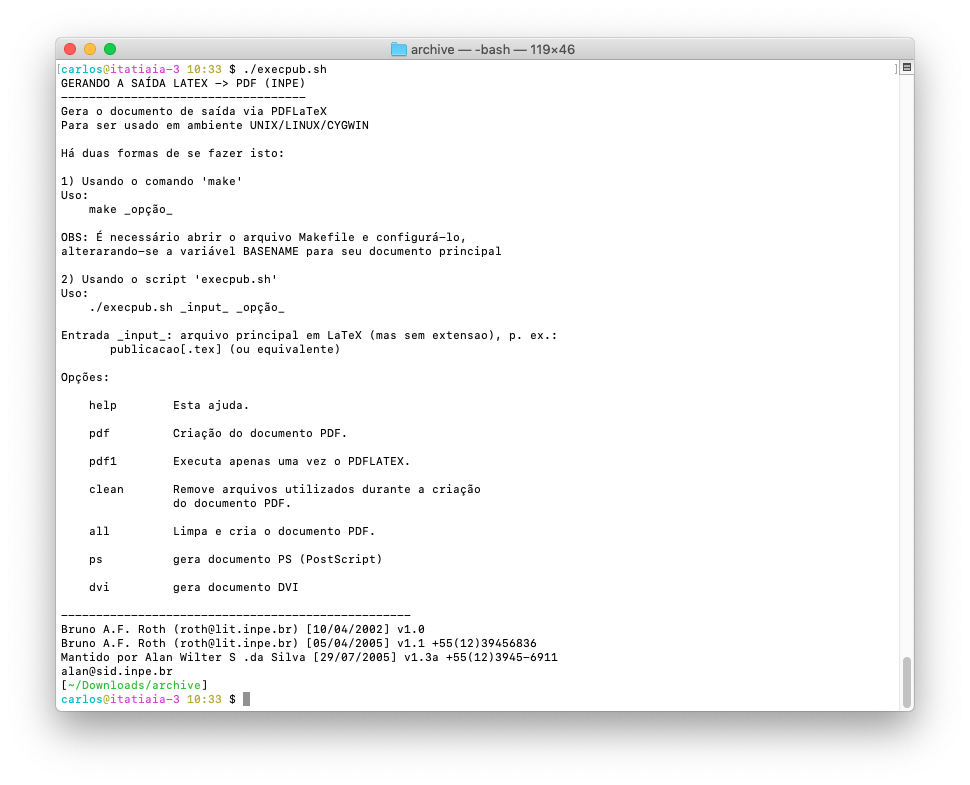
\includegraphics[scale=0.4]{./figs/saida_execpub.png}
    \caption{Exemplo de execução do \textit{script} ``execpub.sh'' sem argumentos.}
    \label{fig:execpub}
\end{figure}

%\begin{commandshell}
%./execpub.sh
%GERANDO A SAÍDA LATEX -> PDF (INPE)
%-----------------------------------
%Gera o documento de saída via PDFLaTeX
%Para ser usado em ambiente UNIX/LINUX/CYGWIN
%
%Há duas formas de se fazer isto:
%
%1) Usando o comando 'make'
%Uso:
%    make _opção_
%
%OBS: É necessário abrir o arquivo Makefile e configurá-lo,
%alterarando-se a variável BASENAME para seu documento principal
%
%2) Usando o script 'execpub.sh'
%Uso:
%    ./execpub.sh _input_ _opção_
%
%Entrada _input_: arquivo principal em LaTeX (mas sem extensao), p. ex.:
%       publicacao[.tex] (ou equivalente)
%
%Opçõess:
%
%    help	Esta ajuda.
%
%    pdf		Criação do documento PDF.
%
%    pdf1	Executa apenas uma vez o PDFLATEX.
%
%    clean	Remove arquivos utilizados durante a criação
%		do documento PDF.
%
%    all		Limpa e cria o documento PDF.
%
%    ps	  	gera documento PS (PostScript)
%
%    dvi		gera documento DVI
%
%--------------------------------------------------
%Bruno A.F. Roth (roth@lit.inpe.br) [10/04/2002] v1.0
%Bruno A.F. Roth (roth@lit.inpe.br) [05/04/2005] v1.1 +55(12)39456836
%Mantido por Alan Wilter S .da Silva [29/07/2005] v1.3a +55(12)3945-6911
%alan@sid.inpe.br
%\end{commandshell}

\textbf{4.} Execute o \textit{script} ``execpub.sh'', com dois argumentos:
\begin{commandshell}
./execpub.sh <arquivo> <opcao>
\end{commandshell}

No comando acima, observe que o nome do arquivo a ser compilado deve ser informado sem a extensão ``.tex''.

Para finalmente compilar o documento principal ``publicacao.tex'', siga o exemplo abaixo. Observe que apenas este comando é necessário para gerar o arquivo PDF final (``publicacao.pdf'').

\textbf{5.} Execute o \textit{script} ``execpub.sh'', com dois argumentos:
\begin{commandshell}
./execpub.sh publicacao pdf
\end{commandshell}

Muitos exemplos estão disponíveis na internet, assim como arquivos \LaTeX{} escritos há muito tempo e que podem fazer uso de codificações diferentes. Isso pode acarretar na incorreta renderização de caracteres especiais, como acentos. Na Figura \ref{fig:leiame} o arquivo leiame do estilo do INPE (assim como vários dos outros arquivos), foram criados e salvo na codificação ISO-8859-2 (frequentemente utilizado pelos sistemas operacionais até poucos anos atrás). Com a padronização do sistema \textit{Portable Operating System Interface} (POSIX) para UTF-8, pode tornar-se necessário abrir estes arquivos com algum editor de textos (como o Gedit no Linux ou o Textedit no Mac OS) e utilizar a opção ``Salvar como...'' para salvar os arquivos no formato UTF-8. 

\begin{figure}[H]
\centering
\subfigure[Renderização errada\label{fig:leiame1}]{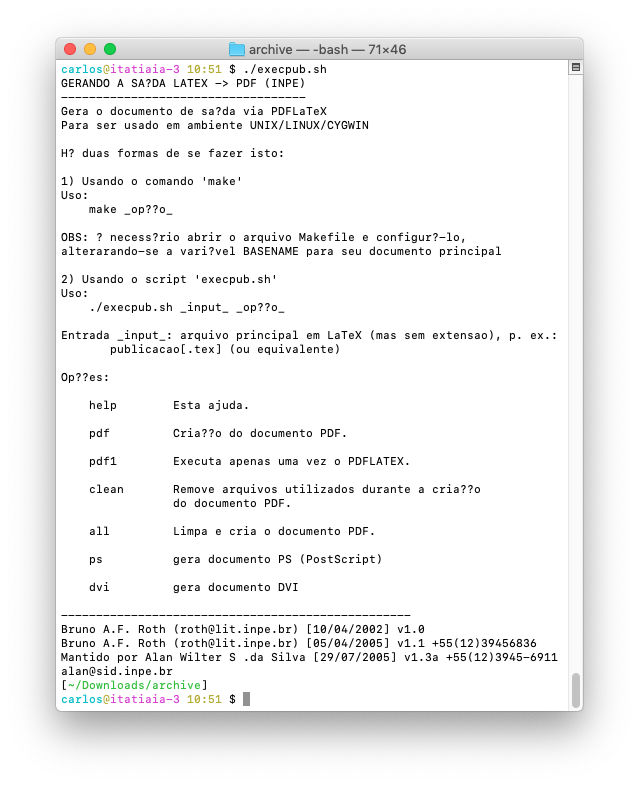
\includegraphics[scale=0.35]{./figs/exemplo_iso8859_1.png}}%\\
\subfigure[Renderização correta\label{fig:leiame2}]{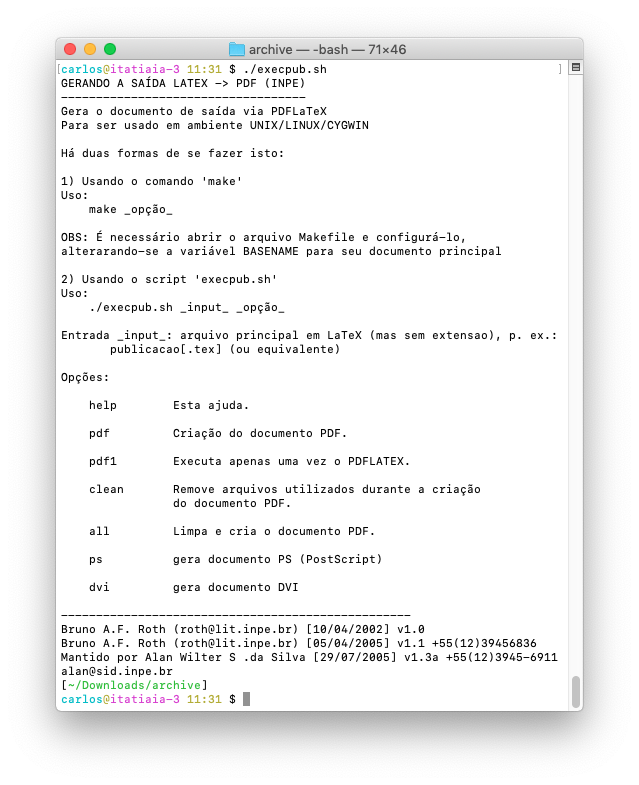
\includegraphics[scale=0.35]{./figs/exemplo_iso8859_3.png}}
\caption{Exemplo da renderização de um arquivo salvo com a codificação ISO-8859-2 em um ambiente UTF-8.}
\label{fig:leiame}
\end{figure}

%\begin{figure}[H]
%\centering
%\begin{subfigure}{.5\textwidth}
%  \centering
%  \includegraphics[scale=0.4]{./figs/exemplo_iso88592_1.png}
%  \caption{A subfigure}
%  \label{fig:sub1}
%\end{subfigure}%
%\begin{subfigure}{.5\textwidth}
%  \centering
%  \includegraphics[scale=0.4]{./figs/exemplo_iso88592_2.png}
%  \caption{A subfigure}
%  \label{fig:sub2}
%\end{subfigure}
%\caption{Exemplo da renderização de um arquivo salvo com a codificação ISO-8859-2 em um ambiente UTF-8.}
%\label{fig:leiame}
%\end{figure}
%
%\begin{figure}%
%    \centering
%    \subfloat[label 1]{{\includegraphics[width=5cm]{img1} }}%
%    \qquad
%    \subfloat[label 2]{{\includegraphics[width=5cm]{img2} }}%
%    \caption{2 Figures side by side}%
%    \label{fig:example}%
%\end{figure}

\begin{marker}
Utilize o comando {\tt iconv} para converter arquivos salvos em codificações diferentes da UTF-8. Para converter um arquivo salvo na codificação ISO-8859-2 para UTF-8, pode-se utilizar o seguinte comando:
\medskip
\begin{commandshell}
iconv -f ISO-8859-9 -t UTF-8 arquivo.tex > novo_arquivo.tex
\end{commandshell}
\medskip
Para mais informações sobre como utilizar o comando {\tt iconv}, digite o comando:
\smallskip
\begin{commandshell}
iconv --help
\end{commandshell}
\end{marker}

\subsection{Arquivos de Configuração}
\label{sec:configura}

No estilo do INPE, há basicamente dois arquivos que devem ser configurados para que o usuário possa definir o nome do(s) autor(es) e o título do documento. São eles:

\begin{itemize}
    \item {\tt publicacao.tex}
    \item {\tt configuracao.tex}
\end{itemize}

No arquivo {\tt publicacao.tex}, são definidos o estilo da publicação, i.e., se o documento terá o estilo de dissertação ou tese ({\tt PublicacaoDissOuTese}, é o padrão), artigo ou relatório ({\tt PublicacaoArtigoOuRelatorio}), proposta de tese ou dissertação ({\tt PublicacaoProposta}), livro com ou sem a formatação de capítulos ({\tt PublicacaoLivro}). Além disso, deve-se ajustar também o idioma: se o idioma principal do documento for o Português, então o abstract será no idioma Inglês ({\tt english, portuguese}), além do tipo de logo do governo e do tipo de licença \textit{Creative Commons} a ser utilizada (veja mais informações em \url{https://pt.wikipedia.org/wiki/Licenças_Creative_Commons}).

%\begin{torntext}[title=Trecho do arquivo {\tt publicacao.tex}]
%$\backslash$\mintinline{latex}{documentclass[\%}
%\\
%\%\%\% PARA ESCOLHER O ESTILO TIRE O SIMBOLO \%(COMENTÁRIO)
%\\
%\%SemVinculoColorido,
%\\
%\%SemFormatacaoCapitulo,
%\\
%\%SemFolhaAprovacao,
%\\
%\%SemImagens,
%\\
%\%CitacaoNumerica, \%\% o padrão é citação tipo autor-data
%\\
%\%PublicacaoDissOuTese, \%\% (é também o "default") com ficha catal. e folha de aprovação em branco. Caso tenha lista de símbolos e lista de siglas e abreviaturas retirar os comentários dos arquivos siglas.tex e abreviaturasesiglas.tex. Retirar também os comentários indicados nesse arquivo, nos includes
%\\
%\%PublicacaoArtigoOuRelatorio, \%\% texto sequencial, sem quebra de páginas nem folhas em branco
%\\
%\%PublicacaoProposta, \%\% igual tese/dissertação, mas sem ficha catal. e fol. de aprov.
%\\
%\%PublicacaoLivro, \%\% com capítulos
%\\
%\%PublicacaoLivro,SemFormatacaoCapitulo, \%\% sem capítulos
%\\
%english,portuguese \%\% para os documentos em Português com abstract.tex em Inglês
%\\
%\%portuguese,english \%\% para os documentos em Inglês com abstract.tex em Português
%\\
%,LogoINPE\% comentar essa linha para fazer aparecer o logo do Governo
%\\
%,CCBYNC	\% as opções de licença são: CCBY, CCBYSA, CCBYND, CCBYNC, CCBYNCSA, CCBYNCND, GPLv3 e INPECopyright
%\\
%]{tdiinpe}
%\\
%\%]{../../../../../iconet.com.br/banon/2008/03.25.01.19/doc/tdiinpe}
%\\
%\% PARA EXIBIR EM ARIAL TIRAR O COMENTÁRIO DAS DUAS LINHAS SEGUINTES
%\\
%\%$\backslash$\mintinline{latex}{renewcommand{\rmdefault}{phv}} \% Arial
%\\
%\%$\backslash$\mintinline{latex}{renewcommand{\sfdefault}{phv}} \% Arial
%\\
%\\
%\% PARA PUBLICAÇÕES EM INGLÊS:
%\\
%\% renomear o arquivo: abnt-alf.bst para abnt-alfportuguese.bst
%\\
%\% renomear o arquivo: abnt-alfenglish.bst para abnt-alf.bst
%\end{torntext}

%\begin{tcboxedraster}[raster columns=3, raster equal height, size=small,colframe=red!50!black,colback=red!10!white,colbacktitle=red!50!white, title={Box \# \thetcbrasternum}] {colback=yellow!10,fonttitle=\bfseries,title=Trecho do arquivo {\tt publicacao.tex}}
%$\backslash$\mintinline{latex}{documentclass[\%}
%\\
%\%\%\% PARA ESCOLHER O ESTILO TIRE O SIMBOLO \%(COMENTÁRIO)
%\\
%\%SemVinculoColorido,
%\\
%\%SemFormatacaoCapitulo,
%\\
%\%SemFolhaAprovacao,
%\\
%\%SemImagens,
%\\
%\%CitacaoNumerica, \%\% o padrão é citação tipo autor-data
%\\
%\%PublicacaoDissOuTese, \%\% (é também o "default") com ficha catal. e folha de aprovação em branco. Caso tenha lista de símbolos e lista de siglas e abreviaturas retirar os comentários dos arquivos siglas.tex e abreviaturasesiglas.tex. Retirar também os comentários indicados nesse arquivo, nos includes
%\\
%\%PublicacaoArtigoOuRelatorio, \%\% texto sequencial, sem quebra de páginas nem folhas em branco
%\\
%\%PublicacaoProposta, \%\% igual tese/dissertação, mas sem ficha catal. e fol. de aprov.
%\\
%\%PublicacaoLivro, \%\% com capítulos
%\\
%\%PublicacaoLivro,SemFormatacaoCapitulo, \%\% sem capítulos
%\\
%english,portuguese \%\% para os documentos em Português com abstract.tex em Inglês
%\\
%\%portuguese,english \%\% para os documentos em Inglês com abstract.tex em Português
%\\
%,LogoINPE\% comentar essa linha para fazer aparecer o logo do Governo
%\\
%,CCBYNC	\% as opções de licença são: CCBY, CCBYSA, CCBYND, CCBYNC, CCBYNCSA, CCBYNCND, GPLv3 e INPECopyright
%\\
%]{tdiinpe}
%\\
%\%]{../../../../../iconet.com.br/banon/2008/03.25.01.19/doc/tdiinpe}
%\\
%\% PARA EXIBIR EM ARIAL TIRAR O COMENTÁRIO DAS DUAS LINHAS SEGUINTES
%\\
%\%$\backslash$\mintinline{latex}{renewcommand{\rmdefault}{phv}} \% Arial
%\\
%\%$\backslash$\mintinline{latex}{renewcommand{\sfdefault}{phv}} \% Arial
%\\
%\\
%\% PARA PUBLICAÇÕES EM INGLÊS:
%\\
%\% renomear o arquivo: abnt-alf.bst para abnt-alfportuguese.bst
%\\
%\% renomear o arquivo: abnt-alfenglish.bst para abnt-alf.bst
%\end{tcboxedraster}

\begin{texexp}{listing only}
documentclass[
% PARA ESCOLHER O ESTILO TIRE O SIMBOLO (COMENTÁRIO)
%SemVinculoColorido,
%SemFormatacaoCapitulo,
%SemFolhaAprovacao,
%SemImagens,
%CitacaoNumerica, 
%PublicacaoDissOuTese,
%PublicacaoArtigoOuRelatorio,
%PublicacaoProposta, 
%PublicacaoLivro, 
%PublicacaoLivro,SemFormatacaoCapitulo,
english,portuguese, 
%portuguese,english, 
LogoINPE,
CCBYNC,
]{tdiinpe}

% PARA EXIBIR EM ARIAL TIRAR O COMENTÁRIO DAS DUAS LINHAS SEGUINTES
%\renewcommand{\rmdefault}{phv}} % Arial
%\renewcommand{\sfdefault}{phv}} % Arial

% PARA PUBLICAÇÕES EM INGLÊS:
%renomear o arquivo: abnt-alf.bst para abnt-alfportuguese.bst
%renomear o arquivo: abnt-alfenglish.bst para abnt-alf.bst
...
\end{texexp}

\begin{table}[H]
\centering
\caption{Configurações principais do arquivo {\tt publicacao.tex}.}
\label{tab:arq_publicacao}
    \begin{tabular}{p{5cm}p{8cm}}
    \hline
    \\[-0.5em]
    \textbf{Opção} & \textbf{Descrição} \\
    \\[-0.5em]
    \hline
    \hline
    \\[-0.5em]
    {\tt SemVinculoColorido}                    & Remove o realce das referências e \textit{links} \\
    \\[-0.5em]
    {\tt SemFormatacaoCapitulo}                 & Não aplica a formatação de capítulos  \\
    \\[-0.5em]
    {\tt SemImagens}                            & Compila o documento sem as imagens \\
    \\[-0.5em]
    {\tt CitacaoNumerica}                       & Altera o estilo das citações \\
    \\[-0.5em]
    {\tt PublicacaoDissOuTese}                  & Aplica o estilo de Dissertação ou Tese \\
    \\[-0.5em]
    {\tt PublicacaoArtigoOuRelatorio}           & Aplica o estilo de Artigo ou Relatório \\
    \\[-0.5em]
    {\tt PublicacaoProposta}                    & Aplica o estilo de Proposta (Tese ou Dissertação) \\
    \\[-0.5em]
    {\tt PublicacaoLivro}                       & Aplica o estilo de Livro \\
    \\[-0.5em]
    {\tt PublicacaoLivro,SemFormatacaoCapitulo} & Idem anterior, mas sem a formatação de catpítulos \\
    \\[-0.5em]
    {\tt english,portuguese}                    & Texto em Português, \textit{Abstract} em Inglês \\
    \\[-0.5em]
    {\tt portuguese,english}                    & Texto em Inglês, Resumo em Português \\
    \\[-0.5em]
    {\tt LogoINPE}                              & Utiliza o logo do INPE ao invés do logo do governo \\
    \\[-0.5em]
    {\tt CCBYNC}                                & Aplica o tipo de licença \\
    \\[-0.5em]
    \mintinline{latex}{\renewcommand{\rmdefault}{phv}}& Aplica a fonte Arial (sem serifa) como padrão \\
%    \\[-0.5em]
%    {\tt LogoINPE}                              & Utiliza o logo do INPE ao invés do logo do governo \\
%    \\[-0.5em]
%    {\tt LogoINPE}                              & Utiliza o logo do INPE ao invés do logo do governo \\
%    \\[-0.5em]
    \hline
    \end{tabular}
\end{table}

%\begin{leaflet}[underlay={\node[above=5mm,font=\footnotesize] 
%    at (frame.south) {- \arabic{tcbbreakpart} -};}]
%     \includegraphics[width=\linewidth]{Basilica_5.png}
%     \begin{center}
%     \bfseries\LARGE Example
%     \end{center}
%     \section{Introduction}
%     \lipsum[1]
%     \section{Main Part A}
%     \lipsum[2-8]
%     \section{Main Part B}
%     \lipsum[9-15]
%     \section{Conclusion}
%     \lipsum[16-18]
%\end{leaflet}

Já no arquivo {\tt configuracao.tex}, o usuário poderá inserir o título do documento, bem como o(s) nome(s) do(s) autor(es) do documento. Outras configurações, são normalmente revisadas e alteradas oportunamente pelo SID.

\begin{texexp}{listing only}
% CAPA
\titulo{Escrever o t\'{i}tulo no idioma em que foi escrito a publicaç\~{a}o}
\title{Escrever o t\'{i}tulo em Ingl\^{e}s para publicaç\~{o}es escritas em Portugu\^{e}s e em Portugu\^{e}s para publicaç\~{o}es escritas em Ingl\^{e}s} 
\author{Nome Completo do Autor}
\descriccao{Tese de Doutorado ou Dissertaç\~{a}o de Mestrado do Curso de P\'{o}s-Graduaç\~{a}o em Nome do Curso, orientada pelo(a) Dr(a). Nome do Orientador(a), aprovada em dd de m\^{e}s por extenso de aaaa.}
\repositorio{aa/bb/cc/dd}
\tipoDaPublicacao{TDI}
\IBI{xx/yy} 
\date{AAAA}
...
\end{texexp}

\begin{marker}
Fique atento para os caracteres que são inseridos no arquivo {\tt configuracao.tex}. Neste arquivo, os acentos devem ser marcados, e.g., a palavra ``{\tt publicação}'', deve ser marcada como ``\mintinline{latex}{publicaç\~{a}o}.''
\end{marker}

%\subsection{Estrutura dos diretórios e arquivos de configuração}
%\subsection{Inclusão de pacotes e suas funções}
%\subsection{Como são divididas as seções}
%\subsection{Introduzindo figuras e gráficos}
%\subsection{Inserindo tabelas e equações}
%\subsection{Citações, Referências Cruzadas e Referências (bibtex, abntex)}
%
%\section{Utilização de Editores}
%\subsection{Linha de comando, editores locais, editor online (Overleaf)}
%
%\section{Ferramentas Úteis}
%\subsection{Construção de tabelas}
%\subsection{Gerenciadores de referências (Mendeley, Zotero)}